% Template LaTeX document for CSSR4A Deliverables
% Adapted from documents prepared by EPFL for the RobotCub project
% and subsequently by the University of Skövde for the DREAM project
%
% DV 28/06/2023

\documentclass{CSSRforAfrica}

%\usepackage[hidelinks,colorlinks=false]{hyperref}
%\usepackage[titletoc,title]{appendix}
%\usepackage{latexsym}

\usepackage[titletoc,title]{appendix}
\usepackage[colorlinks, urlcolor=blue, linkcolor=black, citecolor=black]{hyperref}
\usepackage{latexsym}
\usepackage{comment}
\usepackage{multirow}
\usepackage{subcaption}
\usepackage[breakable,skins,most]{tcolorbox} % Consolidated tcolorbox options
\usepackage{tabularx,colortbl}
\usepackage[tikz]{bclogo} % for boxes
\usepackage{ragged2e}
\usepackage{dirtree}
\usepackage{listings}
\usepackage{textcomp}
\usepackage{natbib}
\usepackage{url}
\usepackage{graphicx}
\usepackage{array}
\usepackage{longtable}
\usepackage{subcaption}
\usepackage{algpseudocode}
\usepackage{csvsimple}
\usepackage{algorithm}
\usepackage{amsfonts}
\graphicspath{ {images/} }

\lstset{upquote=true}
\renewcommand{\DTstyle}{\footnotesize\sffamily}

%%% for listing ; added by Pam %%%%%%%%%%%%%%%%%%%%%%%%%%%%%%
\captionsetup[figure]{format=hang}
\definecolor{codegreen}{rgb}{0,0.6,0}
\definecolor{greenyellow}{rgb}{0.8, 0.7, 0.10}
\definecolor{backcolour}{rgb}{0.95,0.95,0.95} 

\lstdefinestyle{withoutNumbering}{
    backgroundcolor=\color{backcolour},   
    commentstyle=\color{codegreen},
    keywordstyle=\color{magenta},
    stringstyle=\color{codepurple},
    basicstyle=\ttfamily\small,
    breakatwhitespace=false,         
    breaklines=true,                 
    captionpos=b,                    
    keepspaces=true,                 
    showspaces=false,                
    showstringspaces=false,
    showtabs=false,                  
    tabsize=2
}

\newcommand{\blank}{~\\}
\newcommand{\checkbox}{{~~~~~~~\leavevmode \put(-7,-1.5){  \huge $\Box$  }}}

\begin{document}
\input{epsf}

%%
%% SHOULD NOT NEED TO BE CHANGED BEFORE THIS POINT
%% ------------------------------------------------
%%

\deliverable{D5.5.1.1}                  
\title{D5.5.1.1 Gesture Execution}   

\leadpartner{ Carnegie Mellon University Africa}                   
\partner{}                       

\revision{1.2}                     
\deliverabledate{30/09/2024}  
\submissiondate{10/10/2024}   
\revisiondate{04/02/2025}      
\disseminationlevel{PU}
\responsible{Adedayo Akinade }        


%%
%% Create the titlepage
%%

\maketitle
 

\section*{Executive Summary}
%===============================================================
\label{executive_summary}
\addcontentsline{toc}{section}{Executive Summary}
 
Deliverable D5.5.1.1 is focused on developing a comprehensive software module for Gesture Execution, enabling the Pepper robot to perform a range of body and hand gestures. This module encompasses five distinct gesture types: deictic, symbolic, and iconic hand gestures, as well as bowing and nodding body movements. Deictic gestures refer to pointing to specific things in the environment and is important for establishing joint attention  \cite{Bartnecketal2020}. The development process involves approaches to gesture specification, utilising joint space representations for most gestures and Cartesian space for deictic movements. A key feature of this module is its ability to learn gestures through manual teleoperation or human demonstration, employing RGB-D camera technology to map human skeletal movements onto the robot's joint system. This latter functionality is  documented in \href{https://cssr4africa.github.io/deliverables/CSSR4Africa_Deliverable_D5.5.1.2.pdf} {Deliverable D5.5.1.2 Programming by Demonstration}.

The deliverable outlines a software development methodology, including requirements definition, module specification, interface design, module design, coding, and unit testing. Each phase of this process is documented, as outlined in the deliverable. The module integrates with the robot localization system developed in Task 4.2.4, ensuring gesture execution within the robot's environment. This integration is crucial for deictic gestures, where precise pointing in the world frame of reference is essential. Additionally, this module coordinates with the attention subsystem developed in Task 5.3 for controlling the head during diectic gestures to a location. The interface design covers input parameters, output gestures, and control data, specifying appropriate data structures for each gesture type. All coding activities adhere to established software engineering standards as set out in \href{https://cssr4africa.github.io/deliverables/CSSR4Africa_Deliverable_D3.2.pdf} {Deliverable D3.2 Software Engineering Standards Manual}, ensuring high-quality, maintainable code. 

\newpage
 
 
%\graphicspath{{./figs/}}
\pagebreak
\tableofcontents
\newpage


\section{Introduction}
%===============================================================
This document describes the development and implementation of a ROS node for the execution of gestures on the Pepper robot. The gestures include deictic, iconic, symbolic, bow, and nod gestures.
The actuators embedded in Pepper's head enable turn and nod motions, thereby fostering engaging interactions 
through nuanced head movements. The arm and hand actuators give Pepper the capability to mimic human gestures, enhancing its nonverbal communicative and interactive potential. The actuators in the hands further 
permit the opening and closing motions. Such functionality isneeded for projects emphasizing non-verbal communication 
through various gestures and movements.

Moreover, the inclusion of actuators in the torso and hips extends Pepper's mobility, allowing it to perform bends and twists. 
This flexibility is crucial for adapting Pepper's movements to reflect various cultural norms of body language, thereby 
enabling a culturally sensitive interaction. 


\begin{figure}[!hbpt]
\centering
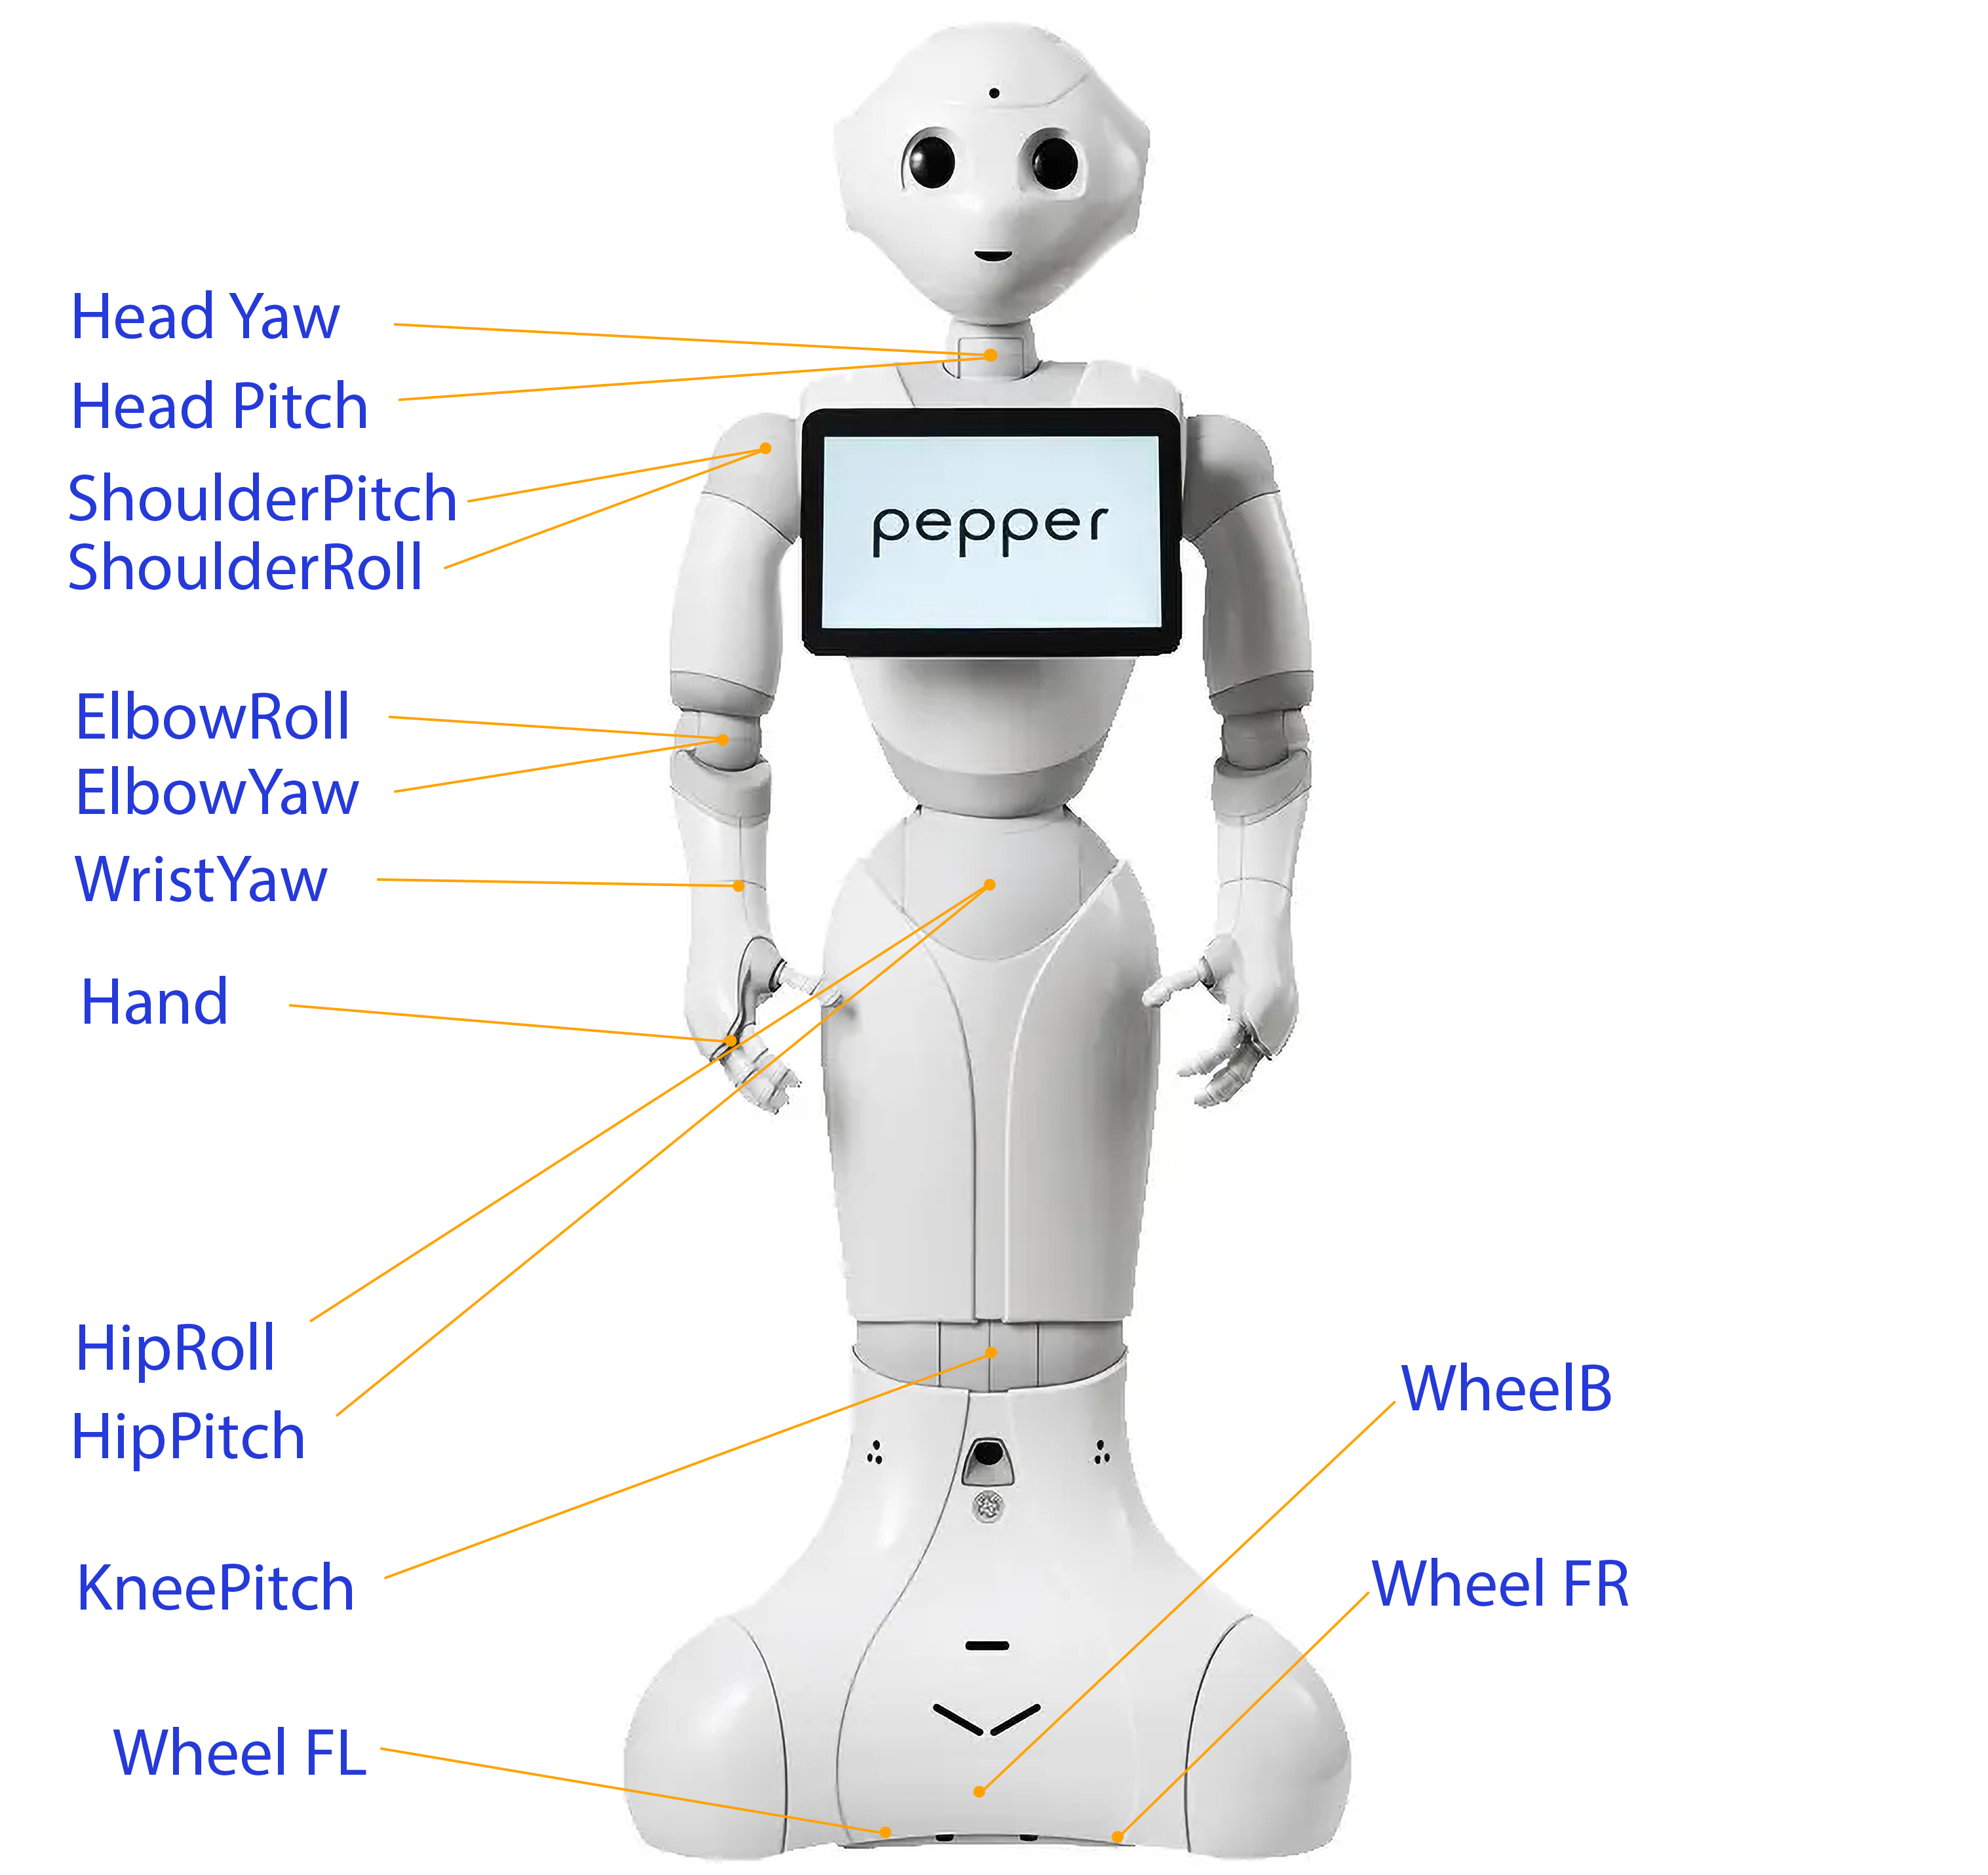
\includegraphics[scale=0.115]{Pepper_actuator.png}
\caption{Pepper robot actuators}
\label{fig:Pepper_actuator}
\end{figure}


This deliverable presents a report that details each phase of the software development lifecycle for our gesture execution system. Section 2 describes the requirements definition process, where functional necessities are aligned with the project's overarching goals. This foundational section establishes the framework upon which subsequent development efforts are built.

Section 3 documents the module specifications, providing details on the execution of gestures. Interface design is then addressed, with particular attention given to data exchange mechanisms utilizing ROS middleware and file input/output operations.

The operational framework of the module is described in Section 4, with a focus on the role of the \texttt{gestureExecutionConfiguration.ini} configuration file in governing system behaviour. This section also outlines the structured approach implemented for handling and processing message data, ensuring efficient and reliable communication within the system. 

Section 5 presents the implemented program code, adhering to the coding standards specified in Deliverable D3.2. This section also provides insights into key algorithms and data structures employed. 

\newpage

 

\section{Requirements Definition}
%===============================================================
The gesture execution provides the robot with the ability to execute five forms of gesture: deictic, symbolic, and iconic non-verbal hand gestures, and bowing and nodding body gestures. This deliverable is important in identifying the specific user expectations, 
ensuring that the node is capable of executing the different gestures in various scenarios, including different
operations and environments (physical robot and simulator). 


As seen from the diagram in Figure \ref{fig:Pepper_actuator}, the Pepper robot has 20 joint actuators and 3 wheel actuators.
The module must be capable of actuating the arm joints to point at a location in the world (for deictic and iconic gestures), actuating the leg joints (for bow gestures), and actuating the head joints (for nod gestures).  If the arm cannot achieve the required pose for a deictic gesture, the robot rotates to make the pose achievable, returning to the original orientation once the gesture is complete. Thus, the module must be capable of actuating the wheels. Furthermore, the arm returns to a neutral position by the robot’s side when the gesture is complete. 

The module must be capable of reading a set of effector waypoints from a file for an iconic gesture and actuating through the points. If an iconic or symbolic gesture involves two arms, they are treated as a composite of two individual gestures, one for each arm.

The pointing location with respect to the robot body, specified by the shoulder pitch and shoulder roll angles, must be computed from the pointing location in the world frame of reference (provided through a service request by a client) and the pose of the robot in the world frame of reference (acquired by subscribing to a topic published by the \texttt{robotLocalization} node). The module must be capable of actuating the joints to achieve the target joint angles, interpolating linearly, or adjusting the joint angles, joint angular velocities, and joint accelerations to mimic biological movement by using a minimum jerk model of biological motion.

The module must be able to run in normal mode or verbose mode. In verbose mode, data that is published to
topics is also printed to the terminal.


\newpage
\section{Module Specification}
%===============================================================

The specifications for these gestures are in joint space, except for deictic gestures which are in
Cartesian space. Some gestures, e.g., iconic and symbolic hand gestures, are specified by learning the required motions either by manual teleoperation, recording the joint angles, or by demonstration, using an RGB-D depth camera to determine the joint angles of human gestures in a skeletal model and mapping these to the robot joints. \href{https://cssr4africa.github.io/deliverables/CSSR4Africa_Deliverable_D5.5.1.2.pdf} {Deliverable D5.5.1.2 Programming by Demonstration} documents the process of learning this gestures by demonstration. Other gestures, i.e., deictic hand gestures and body gestures, are specified by gesture parameters, such as the pointing location for deictic gestures and the degree of inclination for bowing and nodding, and the joint angles are computed using the kinematic model of the robot head, torso, and arms. For deictic gestures, which require the robot to point at objects in its environment, the pose of the robot in the world frame of reference is  used to compute the joint angles while the attention subsystem (documented in \href{https://cssr4africa.github.io/deliverables/CSSR4Africa_Deliverable_D5.3.pdf} {D5.3 Attention Subsystem}) is utilized to control the robot's head to direct its gaze to the location.

Iconic and symbolic gestures are defined by descriptors that specify the final gesture joint configuration and how that configuration is achieved. Descriptors comprise four elements. Each element is a key-value pair, where the value can be an identifier, a number, a vector of numbers, or a vector of a vector of numbers.

The first key-value pair specifies the gesture type (e.g., \texttt{type iconic}, \texttt{type symbolic}).

The second key-value pair identifies the ID number (e.g., \texttt{ID 01}).

The third element defines the number of waypoints in the trajectory, including the start gesture joint configuration and the final gesture joint configuration.

The fourth element is a vector of joint angles vectors. The number of joint angle vectors is equal
to the number of waypoints, including the start joint configuration and the final gesture configuration. Body gestures have three joints: knee pitch, hip pitch, hip roll. Iconic and symbolic gestures have five joints: shoulder pitch, shoulder roll, elbow yaw, elbow roll, and wrist yaw. Before beginning the gesture, the arm is moved from its current joint configuration to the start joint configuration, i.e., the joint angles specified in the first vector in the vector of vector of joint angles.

The number of elements in the vector of joint angles is determined by the gesture type.

Descriptors for each gesture are stored in an external descriptor file.

The joint angles for bow and nod body gestures, as well as hand deictic gestures, are computed at run time using the kinematic model of the robot and the bow angle, nod angle, or the location in the environment to which the robot should point. The bow angle, nod angle, and pointing location are provided as input to the module, along with the time in milliseconds that should elapse between the start of the gesture and the end of the gesture.

The pointing location with respect to the robot body, specified by the shoulder pitch and shoulder roll angles, is computed from the pointing location in the world frame of reference (and supplied as an input to the module) and the pose of the robot in the world frame of reference (provided by the \texttt{robotLocalization} node.  The direction of the robot's gaze is achieved by a ROS service call to the \texttt{overtAttention} node. No waypoints are required for deictic gestures; the joints are actuated to achieve the target joint angles, interpolating linearly, or adjusting the joint angles, joint angular velocities, and joint accelerations to mimic biological movement by using a minimum jerk model of biological motion.

The knee pitch angle is fixed during a bow body gesture and the bow angle corresponds to the change in the hip pitch angle with respect to the default hip pitch angle. Similarly, the nod angle is the change in the head pitch angle with respect to the default head pitch angle. Finally,  the arm and fingers are straight in a deictic gesture, with fixed values of elbow yaw, elbow roll, wrist yaw, and hand angles, so that the palm of the hand is directed upwards, the angles being derived from the pose of the robot with respect to the location to which the robot is gesturing.

The input to the module, as a service request from a client,  is a record comprising the gesture type (e.g., \texttt{iconic}, \texttt{symbolic}, \texttt{deictic}, \texttt{bow}, \texttt{nod}), the gesture ID for symbolic or iconic gestures (e.g., \texttt{01}), the duration of the gesture in milliseconds, and either a bow angle in degrees (for a bow body gesture), or a nod angle in degrees (for a nod body gesture), or the three-dimensional coordinates of a pointing location (for a deictic gesture). For deictic gestures, the module also inputs the current robot pose from the \texttt{robotLocalization} node.

The output of the module is a sequence of joint angles, joint angular velocities, and, optionally, joint angular
accelerations. This output information is compiled into trajectory information, which is sent to the action server created for the appropriate topics, as contained in the topics file for the robot \texttt{robotTopics.dat} and the topics file for the simulator \texttt{simulatorTopics.dat}. The names of the topics to be used for each actuator is read from this data file comprising a sequence of key-value pairs. The key is the name of the actuator. The value is the topic name. There are two data files, one for the physical robot and another for the simulator.  Additionally, the output from the module is a ROS service call to the \texttt{overtAttention} node in the case of a diectic gesture.

The module can run in normal mode or verbose mode. In verbose mode, data that is published to
topics are also printed to the terminal.
 \\~\\

\newpage
\section{Module Design}
%===============================================================



\subsection{Deictic Gestures}

Upon receipt of a service request for a location to point to, the module packages a service request to the \texttt{overtAttention/set\_mode} service to direct the gaze to the location, after which the module employs inverse kinematics to calculate the requisite joint angles for Pepper's arm, enabling precise pointing towards the specified coordinates. This calculation is followed by a validation process to ensure the computed angles fall within the robot's operational limits. The function {\footnotesize \texttt{void get\_arm\_angles(int arm, double elbow\_x, double elbow\_y, double elbow\_z, double wrist\_x, double wrist\_y, double wrist\_z, double* shoulder\_pitch, double* shoulder\_roll, double* elbow\_yaw, double* elbow\_roll)}} takes in the 3D coordinates of the elbow of the robot, which is interpolated based on the lengths of the robot arm, and updates the joint angles for the shoulder and elbow.

A notable feature of this implementation is the optional incorporation of a biological motion model described by \cite{Huberetal2008}. When activated, this model generates trajectories that emulate human-like movements, enhancing the naturalness of the robot's gestures. This feature contributes to the effectiveness of non-verbal communication between the robot and human observers.  The function {\footnotesize \texttt{void compute\_trajectory(std::vector<double> start\_position, std::vector<double> end\_position, int number\_of\_joints, double trajectory\_duration, \\std::vector<std::vector<double>>\& positions, std::vector<std::vector<double>>\& velocities, std::vector<std::vector<double>>\& accelerations, std::vector<double>\& durations)}} compute the trajectory parameters required to move from the default position to that configuration. These trajectory parameters include:
\begin{itemize}
    \item \texttt{positions}: The different positions (joint angles) in the trajectory
    \item \texttt{velocities}: The joint velocities at each waypoint in the trajectory
    \item \texttt{accelerations}: The joint accelerations at each waypoint in the trajectory
    \item \texttt{duations}: the duration of movement between each joint angle in the trajectory
\end{itemize} 


%The execution phase utilises an action server to translate the computed trajectory into physical movement. This server controls Pepper's arm actuators, ensuring the gesture is performed within the specified duration and with the required precision. Throughout the execution, the system continuously monitors the gesture's progress.  
The flow of the gesture execution of a deictic gesture is shown in Figure \ref{fig:architecture} below. Given a location $x_p, y_p, z_p$  in three-dimensional space required to point to, the algorithm for the system is listed in Algorithm \ref{alg:cap} below.

%\newpage
\begin{figure}[h!]
  \centering 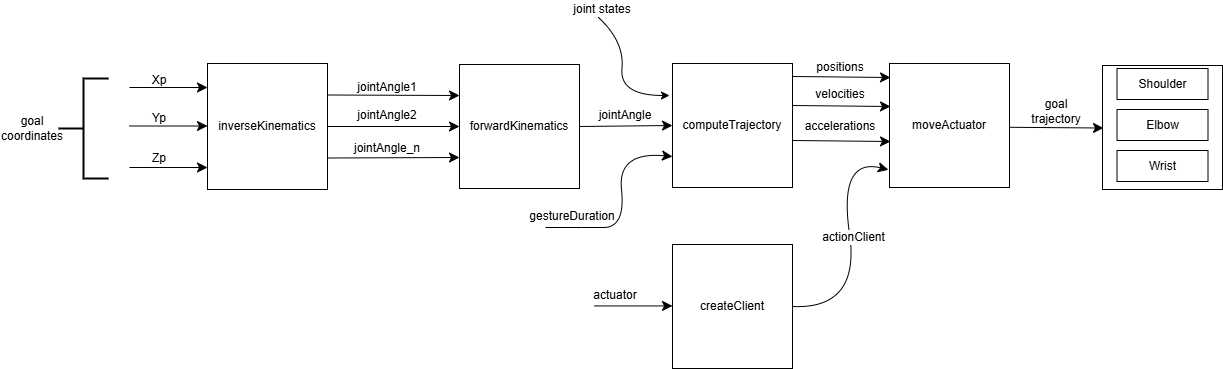
\includegraphics[scale=0.4]{Architecture.png}
  \caption{Architecture of the Gesture Control System for Deictic Gestures}
\label{fig:architecture}
\end{figure}

\newpage
\begin{algorithm}
	\caption{Deictic Gesture Execution Algorithm}\label{alg:cap}
	\begin{algorithmic}
		\Require $biologicalMotionFlag,actuatorJoint, gestureDuration, x_p, y_p, z_p$
		\Ensure $gestureDuration > 0$
		\State $x \gets x_p$
		\State $y \gets y_p$
		\State $z \gets z_p$
		
		\State $jointAngles \gets $ inverseKinematics($x, y, z$) \Comment{Compute the joint angles}
		
		\For{$jointAngle$ in $jointAngles$}
			\State $x_f, y_f, z_f$ = forwardKinematics($jointAngle$) \Comment{Obtain the position}
			\If{$x_f, y_f, z_f = x, y, z$} \Comment{JointAngle is valid}
			    \State break
			\Else
			    \State $status \gets 0$
			    \State return $status$
			\EndIf
		\EndFor
		\State $jointClient \gets $ createClient($actuatorJoint$) \Comment{Create ROS actionClient}
		\If{$biologicalMotionFlag$ is True}
			\State $Positions,Velocities, Accelerations \gets $ computeTrajectory($jointAngle$)
			\State $status \gets $ moveActuator($jointClient,Positions,Velocities, Accelerations$)
		\Else
			\State $status \gets $ moveActuator($jointClient,jointAngle$) \Comment{Move the joint}
		\EndIf
		\State return $status$
	\end{algorithmic}
\end{algorithm}
% \\~\\

\newpage
\subsection{Iconic and Symbolic Gestures}

The specifications for these gestures are in joint space, which are specified in different files for the different gestures. The specifications for the wave gesture descriptors are in the file named \texttt{waveGestureDescriptors.dat}. Welcome gestures are a composite of two arms, thus, the specification for this gesture is in two files \texttt{lArmWelcomeGestureDecriptors} and \\ \texttt{rArmWelcomeGestureDescriptors}.  The specifications in the files contain the information about each gesture. This information includes the ID of the gesture, the number of waypoints (including the start and end joint angle), and the joint angles at each waypoint (delimited by a semicolon). The gestures have been allocated IDs, which are stored in a file named \texttt{gestureDescriptors.dat} and specified in table \ref{tab:Gesture_IDs} below:

\begin{longtable}[c]{|l|l|l|l|}
    \caption{Iconic and Symbolic Gestures and their Allocated IDs} \label{tab:Gesture_IDs} \\
    \hline
    \rowcolor{gray!40}
    \footnotesize{\textbf{ID}} & \footnotesize{\textbf{Gesture}} & \footnotesize{\textbf{Gesture Arm}} &  \footnotesize{\textbf{Descriptor Filename}} \\ \hline
    \endhead % header for subsequent pages
    
   \footnotesize{\texttt{01}} & \footnotesize{\texttt{Welcome Gesture}}  &  \footnotesize{\texttt{Right Arm}} &  \footnotesize{\texttt{rArmWelcomeGestureDescriptors.dat}}  \\ 
   \footnotesize{} & \footnotesize{} &  \footnotesize{\texttt{Left Arm}} & \footnotesize{\texttt{lArmWelcomeGestureDescriptors.dat}}  \\ \hline
   
     \footnotesize{\texttt{02}} & \footnotesize{\texttt{Welcome Gesture}}  &  \footnotesize{\texttt{Right Arm}} &  \footnotesize{\texttt{rArmWelcomeGestureDescriptors.dat}}  \\ 
   \footnotesize{} & \footnotesize{} &  \footnotesize{\texttt{Left Arm}} & \footnotesize{\texttt{lArmWelcomeGestureDescriptors.dat}}  \\ \hline
   
    \footnotesize{\texttt{03}} & \footnotesize{\texttt{Wave Gesture}} &  \footnotesize{\texttt{Right Arm}} &  \footnotesize{\texttt{waveGestureDescriptors.dat}}  \\ \hline
    
    \footnotesize{\texttt{04}} & \footnotesize{\texttt{Shake Gesture}}  &  \footnotesize{\texttt{Right Arm}} &  \footnotesize{\texttt{rArmShakeGestureDescriptors.dat}}  \\ 
   \footnotesize{} & \footnotesize{} &  \footnotesize{\texttt{Left Arm}} & \footnotesize{\texttt{lArmShakeGestureDescriptors.dat}}  \\ \hline
   
   \footnotesize{\texttt{05}} & \footnotesize{\texttt{Shake Gesture}}  &  \footnotesize{\texttt{Right Arm}} &  \footnotesize{\texttt{rArmShakeGestureDescriptors.dat}}  \\ 
   \footnotesize{} & \footnotesize{} &  \footnotesize{\texttt{Left Arm}} & \footnotesize{\texttt{lArmWelcomeShakeDescriptors.dat}}  \\ \hline
    
\end{longtable}

Upon receipt of the service request, the module  reads the descriptor file for the ID requested. The joint angles at each waypoint are read from the file and parsed. If activated, the biological motion model computes the trajectory for the motion through the waypoints. The execution phase utilises an action server to translate the computed trajectory into physical movement. This server controls Pepper's arms, ensuring the gesture is performed within the specified duration and with the required precision. Throughout the execution, the system continuously monitors the gesture's progress.  The flow of the gesture execution of an iconic gesture is shown in Figure \ref{fig:iconicarchitecture} below. Given an ID $gesture\_id$, the algorithm for the system is listed in Algorithm \ref{alg:iconic} below.

\newpage
\begin{figure}[h!]
  \centering 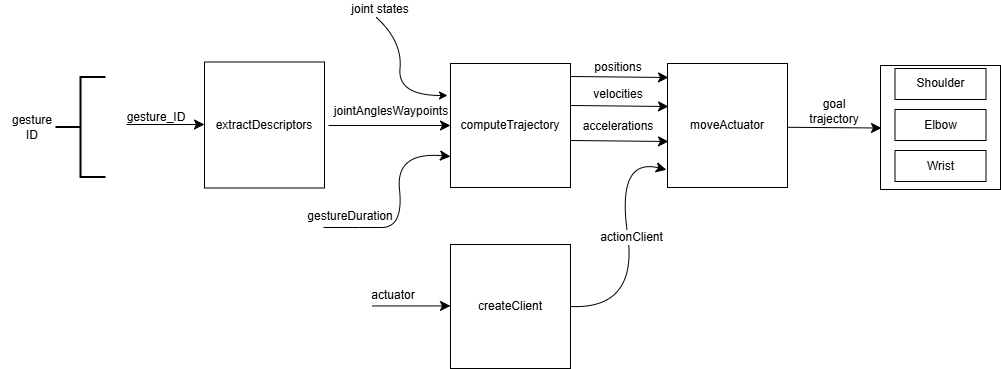
\includegraphics[scale=0.4]{Iconic Architecture.png}
  \caption{Architecture of the Gesture Control System for Iconic Gestures}
\label{fig:iconicarchitecture}
\end{figure}

%\newpage
\begin{algorithm}
	\caption{Iconic Gesture Execution Algorithm}\label{alg:iconic}
	\begin{algorithmic}
		\Require $biologicalMotionFlag,actuatorJoint, gestureDuration, gesture\_id$
		\Ensure $gestureDuration > 0$
		\State $gestureID \gets gesture\_id$
		
		\State $jointAngleWaypoints \gets $ extractDescriptors($gestureID$) \Comment{Extract the waypoints}
		\State $jointClient \gets $ createClient($actuatorJoint$) \Comment{Create ROS actionClient}
		\If{$biologicalMotionFlag$ is True}
			\State $Positions,Velocities, Accelerations \gets $ computeTrajectory($jointAngleWaypoints$)
			\State $status \gets $ moveActuator($jointClient,Positions,Velocities, Accelerations$)
		\Else
			\State $status \gets $ moveActuator($jointClient,jointAngle$) \Comment{Move the joint}
		\EndIf
		\State return $status$
	\end{algorithmic}
\end{algorithm}


Work is being done on specifying the iconic and symbolic hand gestures by learning the required motions either by demonstration, using an RGB-D depth camera to determine the joint angles of human gestures in a skeletal model and mapping these to the robot joints.   This is documented in \href{https://cssr4africa.github.io/deliverables/CSSR4Africa_Deliverable_D5.5.1.2.pdf} {D5.5.1.2 Programming by Demonstration}. 




\newpage
\subsection{Bow Gestures}

Upon receipt of the service request specifying a degree to bow, the module processes the input parameters and if activated, the biological motion model computes the trajectory for the motion. The execution phase utilises an action server to translate the computed trajectory into physical movement. This server controls Pepper's hip and knee joints, ensuring the gesture is performed within the specified duration and with the required precision. Throughout the execution, the system continuously monitors the gesture's progress.  The flow of the gesture execution of a bow gesture is shown in Figure \ref{fig:bowarchitecture} below. Given an angle $theta\_degrees$  in degrees required to bow, the algorithm for the system is listed in Algorithm \ref{alg:bow} below.

%\newpage
\begin{figure}[h!]
  \centering 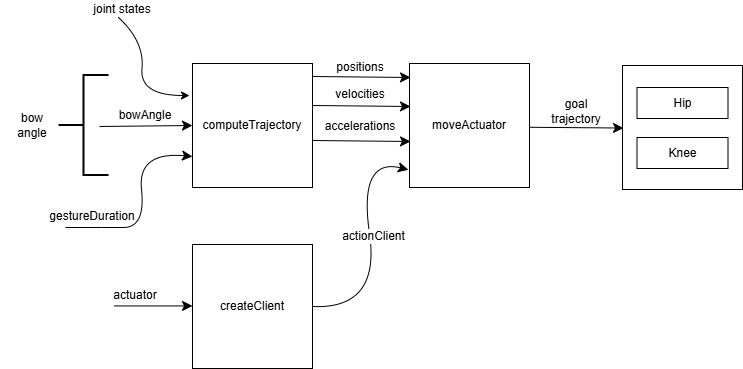
\includegraphics[scale=0.4]{Bow Architecture.png}
  \caption{Architecture of the Gesture Control System for Bow Gestures}
\label{fig:bowarchitecture}
\end{figure}

%\newpage
\begin{algorithm}
	\caption{Bow Gesture Execution Algorithm}\label{alg:bow}
	\begin{algorithmic}
		\Require $biologicalMotionFlag,actuatorJoint, gestureDuration, theta\_degrees$
		\Ensure $gestureDuration > 0$
		\State $jointAngle \gets theta\_degrees$
		
		\State $jointClient \gets $ createClient($actuatorJoint$) \Comment{Create ROS actionClient}
		\If{$biologicalMotionFlag$ is True}
			\State $Positions,Velocities, Accelerations \gets $ computeTrajectory($jointAngle$)
			\State $status \gets $ moveActuator($jointClient,Positions,Velocities, Accelerations$)
		\Else
			\State $status \gets $ moveActuator($jointClient,jointAngle$) \Comment{Move the joint}
		\EndIf
		\State return $status$
	\end{algorithmic}
\end{algorithm}


\newpage
\subsection{Nod Gestures}

Upon receipt of the service request specifying a degree to nod, the module processes the input parameters and if activated, the biological motion model computes the trajectory for the motion.
The execution phase utilises an action server to translate the computed trajectory into physical movement. This server controls Pepper's hip and knee joints, ensuring the gesture is performed within the specified duration and with the required precision. Throughout the execution, the system continuously monitors the gesture's progress.  The flow of the gesture execution of a nodding gesture is shown in Figure \ref{fig:nodarchitecture} below. Given an angle $theta\_degrees$  in degrees required to nod, the algorithm for the system is listed in Algorithm \ref{alg:nod} below. 

%\newpage
\begin{figure}[h!]
  \centering 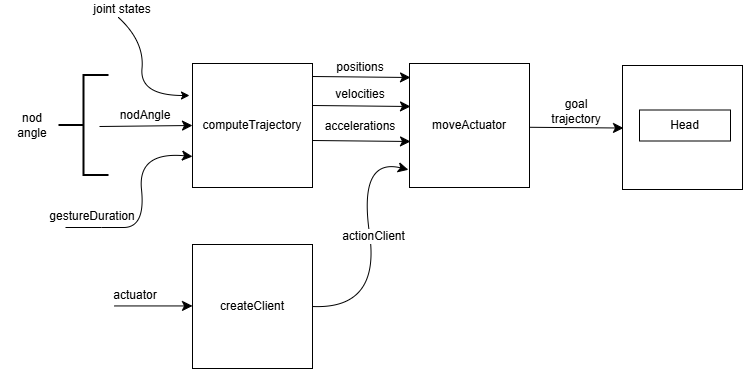
\includegraphics[scale=0.4]{Nod Architecture.png}
  \caption{Architecture of the Gesture Control System for Nod Gestures}
\label{fig:nodarchitecture}
\end{figure}

%\newpage
\begin{algorithm}
	\caption{Nod Gesture Execution Algorithm}\label{alg:nod}
	\begin{algorithmic}
		\Require $biologicalMotionFlag,actuatorJoint, gestureDuration, theta\_degrees$
		\Ensure $gestureDuration > 0$
		\State $jointAngle \gets theta\_degrees$
		
		\State $jointClient \gets $ createClient($actuatorJoint$) \Comment{Create ROS actionClient}
		\If{$biologicalMotionFlag$ is True}
			\State $Positions,Velocities, Accelerations \gets $ computeTrajectory($jointAngle$)
			\State $status \gets $ moveActuator($jointClient,Positions,Velocities, Accelerations$)
		\Else
			\State $status \gets $ moveActuator($jointClient,jointAngle$) \Comment{Move the joint}
		\EndIf
		\State return $status$
	\end{algorithmic}
\end{algorithm}


\newpage
\section{Implementation}
%===============================================================
\subsection*{File Organization}
The source code for executing the gestures is structured into three primary components:
gestureExecutionApplication, gestureExecutionImplementation, and pepperKinematicsUtilitiesImplemmentation. The gestureExecutionImplementation component encapsulates all the essential functionality required for executing the gestures. This includes diectic, iconic, bow, and nod gestures. The gesture execution node is also equipped with the functionality to process various files critical for the execution process, which include configuration files, gesture descriptor files, and
topic files.

On the other hand, the gestureExecutionApplication invokes those functions for the execution process. It is tasked with the execution of functions defined within the gestureExecutionImplementation and pepperKinematicsUtilitiesImplementation, effectively
managing the gesture execution operations.

The file structure of the gesture execution node in the \texttt{cssr\_system} package is shown in Figure \ref{fig:filestructure} below.

%\newpage
\vspace*{0.5em}

\begin{figure}[h!]
\renewcommand*\DTstyle{\ttfamily}
\dirtree{%
.1 cssr\_system.
.2 gestureExecution.
.3 config.
.4 gestureExecutionConfiguration.ini.
.3 data.
.4 gestureDescriptors.dat.
.4 lArmShakeGestureDescriptors.dat.
.4 lArmWelcomeGestureDescriptors.dat.
.4 pepperTopics.dat.
.4 rArmShakeGestureDescriptors.dat.
.4 rArmWelcomeGestureDescriptors.dat.
.4 simulatorTopics.dat.
.4 waveGestureDescriptors.dat.
.3 include.
.4 gestureExecution.
.5 gestureExecutionInterface.h.
.5 pepperKinematicsUtilitiesInterface.h.
.3 launch.
.3 msg.
.4 Gesture.msg.
.3 src.
.4 gestureExecutionApplication.cpp.
.4 gestureExecutionImplementation.cpp.
.4 pepperKinematicsUtilitiesImplementation.cpp.
.3 srv.
.4 performGesture.srv.
.3 README.md.
.3 CMakeLists.txt.
}
 \caption{File Structure for the Gesture Execution Node}
\label{fig:filestructure}
\end{figure}

\newpage

\subsection*{Configuration File}
The operation of the gestureExecution node is determined by the contents of the configuration file that contains a list of key-value pairs as shown below.	

The configuration file is named \texttt{gestureExecutionConfiguration.ini}

% Table of 3 x 4 with the following headers: Key, Value, Description
\begin{longtable}[c]{|l|l|p{7cm}|}
    \caption{Configuration file for the gesture execution node} \label{tab:config_file}\\
    \hline
    \rowcolor{gray!30}
    \small{\textbf{Key}} & \small{\textbf{Value}} & \small{\textbf{Description}} \\ \hline
    \endhead % header for subsequent pages
    

\footnotesize{\texttt{interpolation}} & \footnotesize{\texttt{linear}} or \texttt{biological} & \footnotesize{Specifies the interpolation type. This indicates how the joint angles that define the trajectory in
joint space between the current joint angles and the gesture joint angles are computed for body gesture and hand deictic gestures and between waypoints for iconic and symbolic gestures. The two options are: (a) independent linear interpolation of each joint angle, and (b) biological motion, selecting the sequence of joint angular velocities and joint accelerations to form a trajectory in time and joint space that mimics biological movement.} \\ \hline
 \footnotesize{\texttt{gestureDescriptors}} & \footnotesize{\texttt{gestureDescriptors.dat}}  & \footnotesize{Specifies the filename of the file in which the gesture descriptors are stored. This file contains the information about each iconic gesture descriptor, which includes the ID, the arm to be used and the filename of the file containing the descriptors for the gesture.} \\ \hline
    \footnotesize{\texttt{robotTopics}} & \footnotesize{\texttt{robotTopics.dat}} & \footnotesize{Specifies the filename of the file in which the physical Pepper robot sensor and actuator topic names are stored.} \\ \hline
    \footnotesize{\texttt{simulatorTopics}} & \footnotesize{\texttt{simulatorTopics.dat}} & \footnotesize{Specifies the filename of the file in which the simulator sensor and actuator topic names are stored.} \\ \hline
 \footnotesize{\texttt{verboseMode}} & \footnotesize{\texttt{true}} or \texttt{false} & \footnotesize{Specifies whether diagnostic data is to be printed to the terminal.} \\ \hline
\end{longtable}

\subsection*{Input File}
There is no input data file for the gesture execution node. The gestures are executed based on the service request provided by a client node.

\subsection*{Output Data File}
There is no output data file for the gesture execution node. The result of the gesture execution is returned as a response to the client that invoked the service and diagnostic messages are printed on the screen, depending on the value of \texttt{verboseMode} key in the configuration file.

\subsection*{Topics File}
For the node, a selected list of the topics for the robot and simulator is stored in the topics file. The topic files are written in the .dat file format.
The data file is written in key-value pairs where the key is the actuator name and the value is the topic

The topics file for the robot is named \texttt{robotTopics.dat} and the topics file for the simulator is named \texttt{simulatorTopics.dat}.

\subsubsection*{Topics Subscribed}
This node subscribes to one topic, published by \texttt{robotLocalization} node, which provides the pose
of the robot.

Table \ref{tab:Subscribed_topics} lists the topic to which the \texttt{gestureExecution} node subscribes.
\begin{longtable}[c]{|l|l|l|}
    \caption{Topic Subscribed to by the gestureExecution node.} \label{tab:Subscribed_topics} \\
    \hline
    \rowcolor{gray!30}
    \footnotesize{\textbf{Topic}} & \footnotesize{\textbf{Node}} & \footnotesize{\textbf{Platform}} \\ \hline
    \endhead % header for subsequent pages
    
    \footnotesize{\texttt{/robotLocalization/pose}} & \footnotesize{\texttt{robotLocalization}} & \footnotesize{\texttt{Physical robot}} \\ \hline
\end{longtable}

\subsubsection*{Topics Published}
Table \ref{tab:Published_topics} lists the topics to which the \texttt{gestureExecution} node publishes. These are specified in the files identified by the \texttt{robotTopics} and \texttt{simulatorTopics} key-value pairs in the configuration file.

\begin{longtable}[c]{|l|l|l|}
    \caption{Topics Published by the gestureExecution node.} \label{tab:Published_topics} \\
    \hline
    \rowcolor{gray!30}
    \footnotesize{\textbf{Topic}} & \footnotesize{\textbf{Actuator}} & \footnotesize{\textbf{Platform}} \\ \hline
    \endhead % header for subsequent pages
    
    \footnotesize{\texttt{/pepper\_dcm/LeftArm\_controller/}} & \footnotesize{\texttt{LShoulderPitch, LShoulderRoll,}} & \footnotesize{\texttt{robot}} \\ 
\footnotesize{\texttt{follow\_joint\_trajectory}} & \footnotesize{\texttt{LElbowYaw, LElbowRoll, LWristYaw}} & \footnotesize{} \\ \hline

    \footnotesize{\texttt{/pepper\_dcm/RightArm\_controller/}} & \footnotesize{\texttt{RShoulderPitch, RShoulderRoll,}} & \footnotesize{\texttt{robot}} \\ 
\footnotesize{\texttt{follow\_joint\_trajectory}} & \footnotesize{\texttt{RElbowYaw, RElbowRoll, RWristYaw}} & \footnotesize{} \\ \hline

    \footnotesize{\texttt{/pepper\_dcm/LeftHand\_controller/}} & \footnotesize{\texttt{Left Hand}} & \footnotesize{\texttt{robot}} \\ 
\footnotesize{\texttt{follow\_joint\_trajectory}} & \footnotesize{} & \footnotesize{} \\ \hline

    \footnotesize{\texttt{/pepper\_dcm/RightHand\_controller/}} & \footnotesize{\texttt{Right Hand}} & \footnotesize{\texttt{robot}} \\ 
\footnotesize{\texttt{follow\_joint\_trajectory}} & \footnotesize{} & \footnotesize{} \\ \hline

    \footnotesize{\texttt{/pepper\_dcm/Pelvis\_controller/}} & \footnotesize{\texttt{HipRoll, HipPitch, KneePitch}} & \footnotesize{\texttt{robot}} \\ 
\footnotesize{\texttt{follow\_joint\_trajectory}} & \footnotesize{} & \footnotesize{} \\ \hline

    \footnotesize{\texttt{/pepper\_dcm/cmd\_moveto}} & \footnotesize{\texttt{Wheels}} & \footnotesize{\texttt{robot}} \\ \hline

    \footnotesize{\texttt{/pepper/LeftArm\_controller/}} & \footnotesize{\texttt{LShoulderPitch, LShoulderRoll,}} & \footnotesize{\texttt{simulator}} \\ 
\footnotesize{\texttt{follow\_joint\_trajectory}} & \footnotesize{\texttt{LElbowYaw, LElbowRoll, LWristYaw}} & \footnotesize{} \\ \hline

    \footnotesize{\texttt{/pepper/RightArm\_controller/}} & \footnotesize{\texttt{RShoulderPitch, RShoulderRoll,}} & \footnotesize{\texttt{simulator}} \\ 
\footnotesize{\texttt{follow\_joint\_trajectory}} & \footnotesize{\texttt{RElbowYaw, RElbowRoll}} & \footnotesize{} \\ \hline

    \footnotesize{\texttt{/pepper/Pelvis\_controller/}} & \footnotesize{\texttt{HipRoll, HipPitch, KneePitch}} & \footnotesize{\texttt{simulator}} \\ 
\footnotesize{\texttt{follow\_joint\_trajectory}} & \footnotesize{} & \footnotesize{} \\ \hline

    \footnotesize{\texttt{/pepper/cmd\_vel}} & \footnotesize{\texttt{Wheels}} & \footnotesize{\texttt{simulator}} \\ \hline
\end{longtable}
%
% \\~\\

\newpage

\subsection*{Services Supported}
This node provides and advertizes a server for a service \texttt{/gestureExecution/perform\_gesture} to initiate the performance of a required gesture. It uses a package-specific msg, \texttt{Gesture.msg}. The message has several fields, as follows:

\begin{longtable}[c]{|l|l|l|l|}
    \caption{Fields in the \texttt{Gesture.msg} of the gestureExecution node.} \label{tab:Gesture.msg_field} \\
    \hline
    \rowcolor{gray!30}
    \footnotesize{\textbf{Field}} & \footnotesize{\textbf{Field Value}} & \footnotesize{\textbf{FIeld Type}} & \footnotesize{\textbf{Units}}\\ \hline
    \endhead % header for subsequent pages
    
    \footnotesize{\texttt{gesture\_type}} & \footnotesize{\texttt{iconic, symbolic}} & \footnotesize{\texttt{String}} & \footnotesize{}  \\ 
   \footnotesize{} & \footnotesize{\texttt{deictic, bow, nod}} & \footnotesize{} & \footnotesize{}  \\\hline
\footnotesize{\texttt{gesture\_id}} & \footnotesize{\texttt{<number>}} & \footnotesize{\texttt{Integer}} & \footnotesize{}  \\ \hline
\footnotesize{\texttt{gesture\_duration}} & \footnotesize{\texttt{<number>}} & \footnotesize{\texttt{Integer}} & \footnotesize{\texttt{milliseconds}}  \\ \hline
\footnotesize{\texttt{bow\_nod\_angle}} & \footnotesize{\texttt{<number>}} & \footnotesize{\texttt{Integer}} & \footnotesize{\texttt{degrees}}  \\ \hline
\footnotesize{\texttt{location\_x}} & \footnotesize{\texttt{<number>}} & \footnotesize{\texttt{Real}} & \footnotesize{\texttt{metres}}  \\ \hline
\footnotesize{\texttt{location\_y}} & \footnotesize{\texttt{<number>}} & \footnotesize{\texttt{Real}} & \footnotesize{\texttt{metres}}  \\ \hline
\footnotesize{\texttt{location\_z}} & \footnotesize{\texttt{<number>}} & \footnotesize{\texttt{Real}} & \footnotesize{\texttt{metres}}  \\ \hline
\end{longtable}

If the \texttt{perform\_gesture} request is successful, the service response is “1”; if it is unsuccessful, it is “0”. The service is called by the \texttt{ behaviorController} node.

Table \ref{tab:Supported_services} summarizes the services supported.

\begin{longtable}[c]{|l|l|l|}
    \caption{Service supported by the gestureExecution node.} \label{tab:Supported_services} \\
    \hline
    \rowcolor{gray!30}
    \footnotesize{\textbf{Service}} & \footnotesize{\textbf{Message Value}} & \footnotesize{\textbf{Effect}} \\ \hline
    \endhead % header for subsequent pages
    
   \footnotesize{\texttt{/gestureExecution/perform\_gesture}} & \footnotesize{\texttt{iconic, symbolic}} &  \footnotesize{\texttt{Perform an iconic, symbolic,}}  \\ 
   \footnotesize{} & \footnotesize{\texttt{deictic, bow, nod}} & \footnotesize{\texttt{deictic, bow, or nod gesture}}  \\\hline
\end{longtable}

\subsection*{Services Called}
This node calls the \texttt{/overtAttention/set\_mode} service as shown in Table \ref{tab:Called_services}.


\begin{longtable}[c]{|l|l|l|}
    \caption{Service called by the gestureExecution node.} \label{tab:Called_services} \\
    \hline
    \rowcolor{gray!30}
    \footnotesize{\textbf{Service}} & \footnotesize{\textbf{Message Value}} & \footnotesize{\textbf{Effect}} \\ \hline
    \endhead % header for subsequent pages
    
   \footnotesize{\texttt{/overtAttention/set\_mode}} & \footnotesize{\texttt{mode ("location"), location\_x}} &  \footnotesize{\texttt{Invoke the attention subsystem to}}  \\ 
   \footnotesize{} & \footnotesize{\texttt{location\_y, location\_z}} & \footnotesize{\texttt{look at a location in the world}}  \\\hline
\end{longtable}

The type of variable that is passed as an argument to the \texttt{overtAttention/set\_mode} service and the type of the service call return value is defined in D5.3 Overt Attention.  Specifically, the location mode of the overtAttention node is invoked and the required point coordinates are passed as request in this service call.

\newpage
\section{Executing the Gestures}
%===============================================================
The implementation of the gesture execution node on the Pepper robot is realized as a ROS service \texttt{/gestureExecution/perform\_gesture}, which is hosted and can be called with specific parameters to request the execution of gestures. The service provides a flexible and convenient interface for controlling the robot's gestures, allowing for customization of gesture type, duration, angles of bowing and nodding, as well as the target coordinate for pointing in the world.

The ROS service is invoked with the following parameters:
\begin{itemize}
	\item Gesture Type: the type of gesture to be executed (e.g., \texttt{deictic}, \texttt{iconic}, \texttt{bow}, \texttt{nod}).
	\item Gesture ID: the ID of an iconic gesture to be executed (e.g., \texttt{01}, \texttt{02}, \texttt{03}).
	\item Duration: the duration of the gesture, controlling the speed at which the gesture is performed.
	\item Angle of Bowing: the angle at which the robot should bow if the gesture is bowing.
	\item Angle of Nodding: the angle at which the robot should nod if the gesture is nodding.
	\item Target Coordinate: the target coordinate in the world that the robot should point to, if the gesture is a deictic pointing gesture.
\end{itemize}

\noindent To run the node, the user must run the following command (after waking the robot):


\begin{lstlisting}[style=withoutNumbering, language=bash]
rosrun cssr_system gestureExecution
\end{lstlisting}

{\color{red} 
\noindent \textbf{NOTE:} 
}
The node requires the availability of the \texttt{/rootLocalization/pose} topic and the \\ \texttt{overtAttention/set\_mode} services to run. This services can be made available by one of two ways, outlined below:

\begin{description}
\item[Option 1:]
Running the \texttt{overtAttention} and \texttt{robotLocalization} nodes in \texttt{cssr\_system} package (if available)

\begin{lstlisting}[style=withoutNumbering, language=bash]
rosrun cssr_system robotLocalization
\end{lstlisting}

\begin{lstlisting}[style=withoutNumbering, language=bash]
rosrun cssr_system overtAttention
\end{lstlisting}

\item[Option 2:]
Running the \texttt{gestureExecutionDriver} and \texttt{gestureExecutionStub} nodes in the \texttt{unit\_tests} package and providing the actual robot pose in the physiscal environment

\begin{lstlisting}[style=withoutNumbering, language=bash]
rosrun unit_tests gestureExecutionStub
\end{lstlisting}

\begin{lstlisting}[style=withoutNumbering, language=bash]
rosrun unit_tests gestureExecutionDriver <robot_x> <robot_y>
 <robot_theta>
\end{lstlisting}

\end{description}


After the node is run, the \texttt{/gestureExecution/perform\_gesture} service is available and can be invoked by running the following command:


\begin{lstlisting}[style=withoutNumbering, language=bash]
rosservice call /gestureExecution/perform_gesture -- <gesture_type> <gesture_id> <gesture_duration> <bow_nod_angle> <location_x> <location_y> <location_z>
\end{lstlisting}

 To execute a deictic gesture at a point   \texttt{x\_p, y\_p, z\_p}  for \texttt{T ms}, the user must invoke the service with the command below (replacing the duration and the pointing coordinates with the actual coordinates):

\begin{lstlisting}[style=withoutNumbering, language=bash]
rosservice call /gestureExecution/perform_gesture -- \
deictic 01 T 0 x_p y_p z_p
\end{lstlisting}


 To execute an iconic gesture with gesture ID  \texttt{gesture\_id} for \texttt{T ms}, the user must invoke the service with the command below (replacing the duration and the gesture ID placeholder with the actual parameters):

\begin{lstlisting}[style=withoutNumbering, language=bash]
rosservice call /gestureExecution/perform_gesture -- \
iconic gesture_id T 0 0 0 0
\end{lstlisting}

 To execute a bow gesture at  \texttt{theta\_degrees} for \texttt{T ms}, the user must invoke the service with the command below (replacing the duration and the bow angle placeholder with the actual bow angle):

\begin{lstlisting}[style=withoutNumbering, language=bash]
rosservice call /gestureExecution/perform_gesture -- \
bow 01 T theta_degrees 0 0 0
\end{lstlisting}

To execute a nod gesture at  \texttt{theta\_degrees} for \texttt{T ms}, the user must invoke the service with the command below (replacing the duration and the nod angle placeholder with the actual nod angle):

\begin{lstlisting}[style=withoutNumbering, language=bash]
rosservice call /gestureExecution/perform_gesture --  \
bow 01 T theta_degrees 0 0 0
\end{lstlisting}


For executing gestures on the physical robot, the NAOqi DCM (Device Communication Manager) driver is used to control the robot's actuators. 
The driver provides a hardware interface to connect to Alderban's robot Nao, Romeo, and Pepper robots. The module is designed to move the joint actuator of the robot to a specified position by defining the trajectory goal and sending it to a control server via a ROS topic. 

First, the module initializes a client for interacting with the ROS actions server. The function is a structured attempt to establish a connection with the server. The connection to the server is attempted multiple times before giving up and throwing an error. The function \\ {\footnotesize \texttt{ControlClientPtr 
create\_client(const std::string\& topic\_name)}} takes in the topic name and returns the actionClient pointer. 

After the client is created, the module commands the robot to move to a specified position by defining a trajectory
goal and sending it to the control server via the ROS action client. First, the module defines a goal message for 
a joint trajectory action, which is part of the \texttt{control\_msgs} package. The \texttt{follow\_joint\_trajectory}
action is used to generate a more complex motion control mechanism, often used for executing predefined paths or
trajectories for a set of joints. 

The components of this topic include: 
\begin{itemize}
    \item \texttt{/goal}: used to send a ``FollowJointTrajectoryGoal", which includes a trajectory comprising multiple points (position, 
    velocities, acceleration, and/or efforts for each joint) and the time at which those points should be reached.
    \item \texttt{/cancel}: can cancel a currently executing trajectory.
    \item \texttt{/feedback}: provides real-time feedback about the current state of the trajectory 
    execution. 
    \item \texttt{/result}: provides the outcome of the trajectory execution after completion.
    \item \texttt{/status}: provides status information about the goal, such as if it's active, succeeded, or aborted
\end{itemize} 

The trajectory goal is sent to the action server through the client. The server, presumably a part of a 
motion control system, interprets this goal and commands the robot arm to move accordingly. The system 
then waits for a fixed duration for the movement to complete before proceeding.

\newpage
\section{Unit Tests}
%===============================================================

To start the unit tests, the user must first install the necessary software packages as outlined in \href{https://cssr4africa.github.io/deliverables/CSSR4Africa_Deliverable_D3.3.pdf}
{Deliverable D3.3}. The operation of the unit test is controlled by a configuration file \\ \texttt{gestureExecutionTestConfiguration.ini} which contain key-value pairs required to execute the unit tests as shown below. 

\begin{longtable}[c]{|l|l|p{7cm}|}
    \caption{Configuration file for the gesture execution unit tests node} \label{tab:unit_tests_config_file}\\
    \hline
    \rowcolor{gray!30}
    \small{\textbf{Key}} & \small{\textbf{Value}} & \small{\textbf{Description}} \\ \hline
    \endhead % header for subsequent pages

    
\small{\texttt{iconic}} & \small{\texttt{true}} or \texttt{false} & \small{Specifies whether to run the iconic gestures test} \\ \hline

\small{\texttt{deictic}} & \small{\texttt{true}} or \texttt{false} & \small{Specifies whether to run the deictic gestures test} \\ \hline
 
\small{\texttt{bow}} & \small{\texttt{true}} or \texttt{false} & \small{Specifies whether to run the bow gestures test} \\ \hline
    
\small{\texttt{nod}} & \small{\texttt{true}} or \texttt{false} & \small{Specifies whether to run the nod gestures test} \\ \hline
    
 \small{\texttt{verboseMode}} & \small{\texttt{true}} or \texttt{false} & \small{Specifies whether diagnostic data is to be printed to the terminal.} \\ \hline


\end{longtable}


Referring to Table \ref{tab:unit_tests_config_file} above, the user must specify which gestures to test using the key-value pairs, with the gesture type (\texttt{deictic}, \texttt{iconic}, \texttt{bow} and \texttt{nod}) as the key and the status (\texttt{True} or \texttt{False}) as the value. To launch the gesture execution test, the user must run the following commands:

\begin{lstlisting}[style=withoutNumbering, language=bash]
# Launch the physical robot
roslaunch unit_tests gestureExecutionLaunchRobot.launch \
robot_ip:=<robot_ip> roscore_ip:=<roscore_ip> \
network_interface:=<network_interface>
\end{lstlisting}


\begin{lstlisting}[style=withoutNumbering, language=bash]
# Launch the physical robot
roslaunch unit_tests gestureExecutionLaunchTestHarness.launch \
launch_drivers_stubs:=true launch_test:=true initial_robot_x:=<robot_x>
initial_robot_y:=<robot_y> initial_robot_theta:=<robot_theta>
\end{lstlisting}



The above commands will launch the test for the robot. The unit tests wake up the robot, launch the gesture execution node (to make the \texttt{gestureExecution/perform\_gesture} service available), launch a driver for the robotLocalization node (to publish the pose of the robot) and launch a stub for the \texttt{/overtAttention/set\_mode} service which randomly returns success or failure when the gesture execution node invokes the service. Based on the status of the gesture being executed, this result is saved in a file \texttt{gestureExecutionTestOutput.dat}. This file stores the input requirement for each gesture and the status of the gesture (either \texttt{Success} or \texttt{Failure}). \\~\\

{\color{red}
\noindent \textbf{NOTE:}
}
Setting the argument \texttt{launch\_test} to \texttt{true} runs the tests based on the configuration, while setting it to \texttt{false} only launches the node and its dependencies. This is particularly useful if the user wants to run unique tests on the node, which are not available in this document. Setting the argument \texttt{launch\_drivers\_stubs} to \texttt{true} launches the drivers and stubs required to drive the \texttt{gestureExecution} node from the \texttt{unit\_tests} package, while setting it to \texttt{false} launches the actual nodes (if available) which include \texttt{faceDetection},  \texttt{soundDetection},  \texttt{overtAttention}, and  \texttt{robotLocalization} from the  \texttt{cssr\_system} package. The default values are  \texttt{true}. Ensure that the robot pose matches the exact pose of the robot in the world frame of reference.






\newpage
%\nocite{*}
\bibliographystyle{unsrt}
%================================================================
\bibliography{cognitive_systems.bib}                                     % REPLACE with correct filename
\addcontentsline{toc}{section}{References}



\pagebreak
\section*{Principal Contributors}
%===============================================================
\label{contributors}
\addcontentsline{toc}{section}{Principal Contributors}
The main authors of this deliverable are as follows (in alphabetical order).
\blank
~
\blank
Adedayo Akinade, Carnegie Mellon University Africa.\\ 
David Vernon, Carnegie Mellon University Africa.\\   

 

  

\newpage
\section*{Document History}
%================================================================
\addcontentsline{toc}{section}{Document History}
\label{document_history}

\begin{description}

\item [Version 1.0]~\\
First draft. \\
Adedayo  Akinade. \\            
10 October 2024                                          
\item [Version 1.1]~\\
Renumbered to D5.5.1.1 to facilitate an additional deliverable for Task 5.5.1: D5.5.1.2  Programming by Demonstration.\\
David Vernon. \\                                   
6 January 2025.   

\item [Version 1.2]~\\
Removed all references to simulator platform, provided additional information on running the unit tests, and added hyperlinks to relevant external documentation.\\
Adedayo Akinade. \\                                   
4 February 2025.   

\end{description}

\end{document}

